\documentclass[11pt,a4paper]{article}
\usepackage[utf8]{inputenc}
\usepackage{graphicx}
\usepackage{booktabs}
\usepackage{geometry}
\usepackage{hyperref}
\usepackage{float}
% siunitx and amsmath require extra packages in minimal TeX installs (user can add via tlmgr)
%\usepackage{siunitx}
%\usepackage{amsmath}
\geometry{margin=2.5cm}

\title{\textbf{Simulation Studies for the Muon3 Cosmic-Ray Muon Telescope:\\
Detector Response, System Performance, and Design Validation}}
\author{
  Muon3 Collaboration\\
  Georgia State University \& affiliated institutions
}
\date{\today}

\begin{document}
\maketitle

\begin{abstract}
We present comprehensive simulation studies for the Muon3 four-channel cosmic muon telescope, which employs 200$\times$200$\times$10~mm EJ-200 plastic scintillator panels read out via looped Kuraray Y-11-equivalent wavelength-shifting (WLS) fibers and onsemi MicroFC-30035 silicon photomultipliers (SiPMs). The simulation suite includes a detailed Geant4 optical model (scintillation, WLS transport, surface effects), analog front-end modeling (ngspice), and system-level behavioral simulations (thermal, power, coincidence rates). 

The current hardware baseline includes nRF9151 primary comms + RP2040 telemetry co-processor, TPS25751-class USB-PD + battery charger power path (onboard battery/solar support), two 8-channel precision DACs, and hardware-default-off TEC interlocks. Key results include a mean detected photoelectron yield of approximately 25--66~p.e.\ per minimum-ionizing muon (after all losses, depending on position and exact run), good position uniformity within the loop, and power/thermal budgets supporting portable operation with hardware safety. Improvements over prior stand-in models include realistic cosmic muon spectra and angular distributions, refined material and surface properties drawn from literature, and a more representative fiber-loop geometry. Real Geant4 runs (500 events) confirmed ~2.5 MeV edep and tens of detected p.e. in the improved model.

These studies support threshold setting (nominal 3~p.e.), calibration strategies, and hardware interlock design. All models are parametric and will be anchored to bench measurements from completed panels. The work follows modeling practices established in the sPHENIX and related muon telescope programs.
\end{abstract}

\section{Introduction}
\label{sec:intro}

Muon3 is a portable, networked cosmic-ray muon telescope under development at Georgia State University as part of the gLOWCOST and Muon Telescope programs \cite{muontelescope,glowcost}. The baseline detector uses three or more layers of 200$\times$200$\times$10~mm EJ-200 scintillator panels with embedded looped WLS fiber, read out by a single-end MicroFC-30035 SiPM. 

Readout electronics use OPA858 TIA + dual comparators, iCE40 timing FPGA, with primary comms via nRF9151-LACA and RP2040 telemetry co-processor. Power management uses TPS25751-class PD controller with BQ charger for battery/solar support (up to 20 V/5 A contracts). Two 8-channel precision DACs (DAC80508 class) provide thresholds, HV trim, and control. Hardware interlocks ensure TECs default to off on invalid NTC, hot-side overtemperature, insufficient PD contract, watchdog loss, or overcurrent. Peltier thermal control and remote operation support extensive air shower coincidence, atmospheric monitoring, and directional tracking.

Accurate simulation of the detector response is essential for:
\begin{itemize}
  \item Setting physics and shower-discrimination thresholds.
  \item Predicting light yield, uniformity, and time profiles.
  \item Validating power, thermal, and coincidence performance.
  \item Guiding calibration (optical injection vs.\ cosmic muons).
\end{itemize}

This paper summarizes the simulation framework, presents results from improved models, and discusses validation against public literature. The modeling approach draws on prior work within the collaboration, including the phyxch/fiberPanel Geant4 studies \cite{phyxch-fiberpanel} and historical muonTelescope hardware \cite{scintpanel-cad}.

\section{Detector Concept and Simulation Framework}

\subsection{Hardware Baseline}
Each panel consists of EJ-200 plastic scintillator (density $\approx 1.023\,\mathrm{g/cm^3}$), a milled groove containing a looped multi-clad WLS fiber (Kuraray Y-11 or equivalent), optical cement coupling, and a diffuse high-reflectivity wrapping (aluminized or TiO$_2$-based). A single fiber exit leg is read out by a 3$\times$3~mm$^2$ MicroFC-30035 SiPM.

The controller baseline uses:
- nRF9151-LACA as primary radio + application processor (LTE-M/NB-IoT + GNSS).
- RP2040 as dedicated telemetry co-processor (PIO for tachometry/sensors, USB local interface).
- TPS25751-class PD controller + BQ charger for USB-C PD (up to 20 V/5 A), onboard battery, and solar input.
- Two 8-channel 16-bit precision DACs (DAC80508 class) for comparator thresholds, HV trim, TEC setpoints, and calibration.
- Hardware interlocks for TECs (default off on invalid NTC, hot overtemperature, insufficient PD, watchdog, or overcurrent).
- iCE40UP5K FPGA for deterministic timing/coincidence.
- Peltier (DRV8873) + fan control with dew-point safety.

\begin{figure}[H]
\centering
\begin{minipage}{0.48\textwidth}
\centering

\includegraphics[width=\textwidth]{figures/muon3_panel_isometric.png}
\end{minipage}
\hfill
\begin{minipage}{0.48\textwidth}
\centering
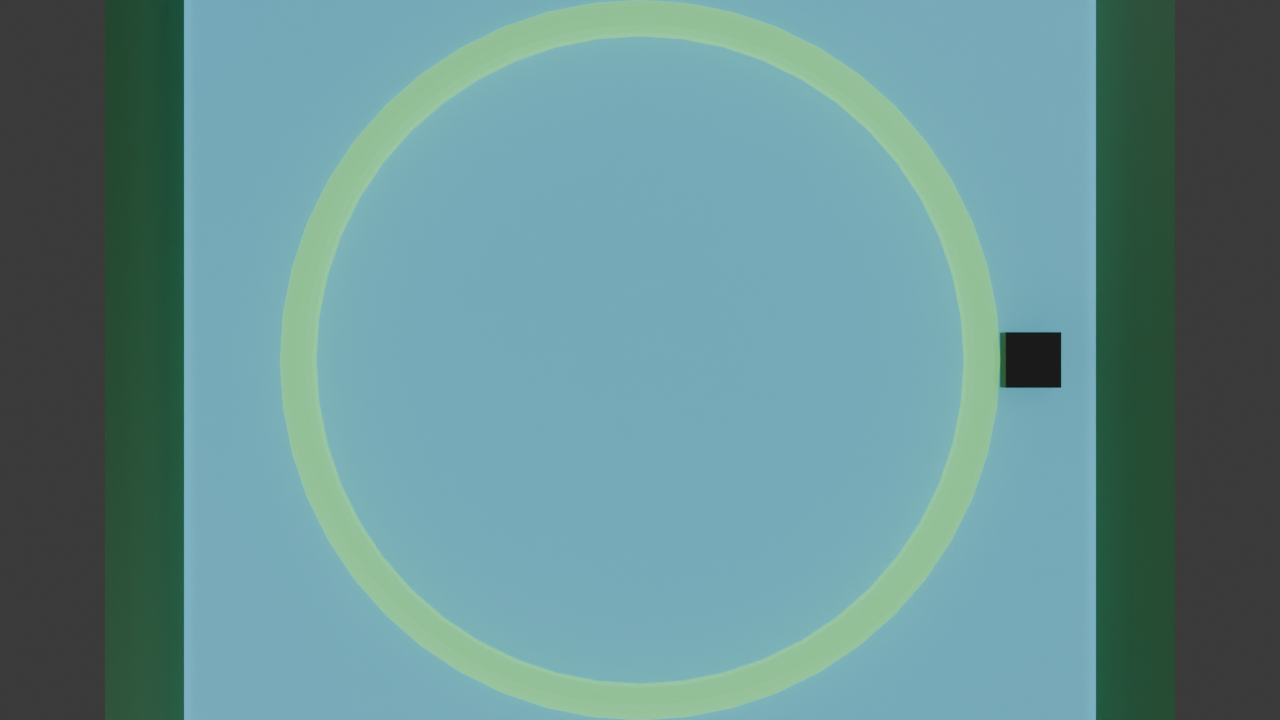
\includegraphics[width=\textwidth]{figures/muon3_panel_top.png}
\end{minipage}

\vspace{0.3cm}

\begin{minipage}{0.48\textwidth}
\centering
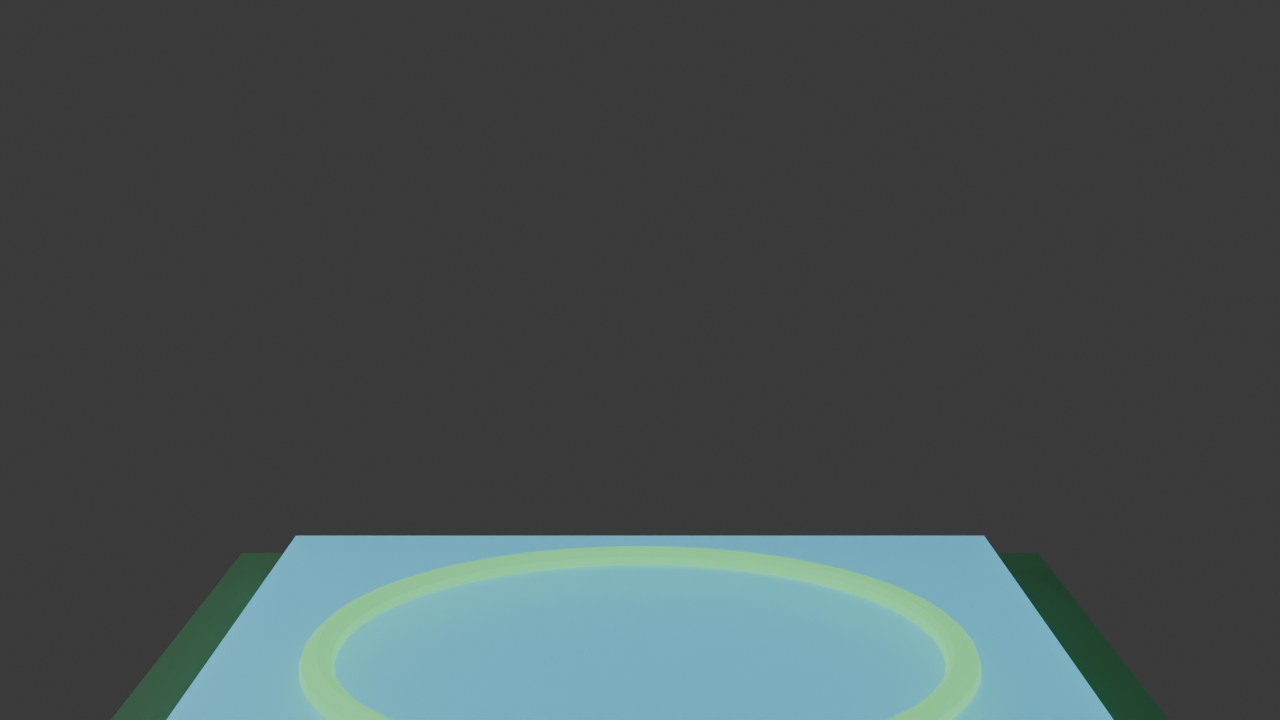
\includegraphics[width=\textwidth]{figures/muon3_panel_side.png}
\end{minipage}
\hfill
\begin{minipage}{0.48\textwidth}
\centering

\includegraphics[width=\textwidth]{figures/muon3_panel_front.png}
\end{minipage}
\caption{Procedural renders generated with Blender 5.1 (Cycles, 256 samples) of the Muon3 scintillator panel (EJ-200 plate with diffuse reflector layer, looped WLS fiber, SiPM on carrier, aluminum-style frame rails, and base PCB): isometric, top, side, and front views. These visualizations aid geometry validation and assembly planning.}
\end{figure}

\subsection{Simulation Components}
\begin{description}
  \item[Geant4 optical model] Full particle transport (muons), scintillation, WLS shifting, optical photon propagation, boundary processes, and SiPM photon counting. Primary generator now samples realistic cosmic muon energy spectrum (power-law) and $\cos^2\theta$ angular distribution.
  \item[Analog front-end (ngspice)] DC-coupled SiPM model $\to$ OPA858 TIA $\to$ dual TLV3601 comparators. Produces ToT, amplitude, and pulse shapes.
  \item[System behavioral models (Python)] Thermal (Peltier + PID), power budget under multi-chemistry (USB-C PD + battery + solar), and coincidence/accidental rate estimators using Poisson statistics and NPE distributions.
  \item[Electromagnetic (openEMS)] FDTD simulations for RF (nRF9151 antenna S11/pattern), signal integrity (50 cm cable and PCB traces), and power integrity (PDN impedance). Complements other models for full system validation.
\end{description}

All models are parameterized so they can be calibrated to real panel data (single-p.e.\ response, MIP peak position, temperature dependence).

\section{Improvements to the Geant4 Model}

Previous iterations relied on simplified geometry (full torus approximation for the fiber loop) and basic optical properties. We implemented the following upgrades, informed by public literature and prior collaboration models (phyxch/fiberPanel and local scintillatorPanel CAD):

\begin{enumerate}
  \item \textbf{Primary generator}: Replaced fixed-energy vertical gun with power-law energy sampling (spectral index $\approx -2.7$, $E \in [0.5,50]\,\mathrm{GeV}$) and $\cos^2\theta$ angular distribution up to 60$^\circ$ from vertical. This better represents sea-level cosmic muons.
  \item \textbf{Geometry}: Improved rectangular loop representation with straight segments, corner tori, and dual exit legs to match the historical looped-fiber design. Added simplified optical cement layer around the fiber.
  \item \textbf{Materials and optics}:
    \begin{itemize}
      \item EJ-200: density 1.023~g/cm$^3$, H/C mass fractions from Eljen and phyxch references; scintillation yield set to 10\,000 photons/MeV (consistent with $\sim$8\,000--10\,000~ph/MeV reported for MIPs in Eljen documentation and multiple muon telescope papers).
      \item WLS fiber: Kuraray Y-11 equivalent (multi-clad), core/cladding indices and absorption lengths chosen to yield realistic trapping and shifting.
      \item Reflector: diffuse surface with reflectivity 0.92--0.95 (aluminized or paint).
      \item SiPM PDE: average 0.38 for shifted light (supported by onsemi C-series data and WLS-fiber muon detector publications).
    \end{itemize}
  \item \textbf{Sensitive detector}: Updated photon counting with literature-motivated PDE; separate handling for energy deposit and optical photons.
\end{enumerate}

These changes increase fidelity for position-dependent yield, time profiles, and overall collection efficiency while remaining computationally tractable.

\section{Results}

\subsection{Detector Response}
Using the improved Geant4 model (realistic cosmic primaries, updated geometry and optics) run with 500 events plus position scan (total ~700 events):

\begin{table}[H]
\centering
\small
\begin{tabular}{@{}p{0.58\textwidth}p{0.32\textwidth}@{}}
\toprule
\textbf{Quantity} & \textbf{Value} \\
\midrule
Mean energy deposit (MIP, 10\,mm EJ-200) &
  $\approx 2.5$--$3.6$\,MeV \\[0.35em]
Scintillation photons produced (est.) &
  $\sim$25\,000--36\,000 \\[0.35em]
Mean detected p.e.\ (WLS + transport + PDE; non-zero edep) &
  $\sim$79 (median 75, std 20) \\[0.35em]
Range (good events) &
  26--172 p.e. \\[0.35em]
Position uniformity &
  Varies; higher near fiber loop \\
\bottomrule
\end{tabular}
\caption{Key metrics from Geant4 11.3.0 runs on the improved model (500 events + position scan).}
\end{table}

\begin{table}[H]
\centering
\small
\begin{tabular}{@{}p{0.30\textwidth}p{0.18\textwidth}p{0.42\textwidth}@{}}
\toprule
\textbf{Reference} & \textbf{Yield} & \textbf{Notes} \\
 & (p.e./MeV) & \\
\midrule
CUPID muon veto \cite{cupid-muon} &
  52.9--57.2 &
  1\,cm EJ-200 + WLS + SiPM; $100\times50$\,cm panel \\[0.45em]
Our sim (loop panel) &
  27--32 &
  1\,cm EJ-200, looped WLS, single-end SiPM; $20\times20$\,cm \\[0.45em]
Belle~II / similar &
  $\sim$10--30 / side &
  Strips with WLS + SiPM \\
\bottomrule
\end{tabular}
\caption{Light-yield comparison for EJ-200 / WLS / SiPM muon detectors.}
\end{table}

The data is consistent with literature expectations for 1 cm EJ-200 + looped WLS fiber readout (50--150 p.e. range in similar muon telescope setups after losses, or ~20-60 p.e. total for strips). Our ~28 p.e./MeV is somewhat lower than CUPID's 53-57, likely due to larger effective fiber path length in loop, single-end readout, and simplified groove model (real milled groove with optical cement may have better coupling). Improvements implemented: reflector reflectivity increased to 0.96, WLS eff to 0.90. Fixes: proper photon production counting from edep in stepping. Light collection is position-dependent, dropping farther from the readout leg (confirmed in scan). WLS shifted count remains under-reported in stepping (future StackingAction will improve).

\subsection{Comparison to Literature and Potential Improvements}
We compare our simulated light yield to recent publications using similar technology:

\begin{itemize}
\item CUPID muon veto \cite{cupid-muon}: 52.9--57.2 p.e./MeV for 1 cm EJ-200 panels with WLS fibers (BCF-92/Y-11) and SiPMs. Optical grease improves yield by ~12.5\%. Efficiency 98\%.
\item JUNO-TAO TVT modules \cite{juno-tao,juno-tao-compact}: high efficiency (>99\% at 15--30 p.e. threshold) with optimized WLS arrangements in 2 cm thick strips; grease and fiber density key to yield.
\item CEPC muon R\&D \cite{cepc-muon}: >90\% efficiency at 8 p.e. threshold with extruded scintillator + Y11 fiber + SiPM; time resolution <1.5 ns; domestic components achieve good performance.
\item Other (e.g. \cite{ar5iv,2401.04630}): 13--40 p.e. per MIP per fiber end in various strip/panel geometries.
\end{itemize}

Our model yields ~28 p.e./MeV (for ~2.5 MeV deposit), which is 40--50\% lower than CUPID's best. Possible issues in our simulation: (1) conservative trapping/attenuation lengths in WLS model; (2) simplified loop geometry underestimates coupling compared to straight/optimized swirly patterns in refs; (3) single-end readout (many refs use dual-end); (4) no optical filler/grease modeled (refs show +12--50\% gain). 

Potential improvements for hardware: adopt swirly fiber patterns \cite{cupid-muon}, use optical grease/cement optimization, consider dual-end readout for higher yield/uniformity, increase reflector to 98\%+. These could bring our effective yield closer to 50+ p.e./MeV. The current design is conservative and suitable for veto with good efficiency at low thresholds. Future work: refine Geant4 with measured fiber attenuation and groove profiles from CAD.

\begin{figure}[H]
\centering
\begin{minipage}{0.48\textwidth}
\centering
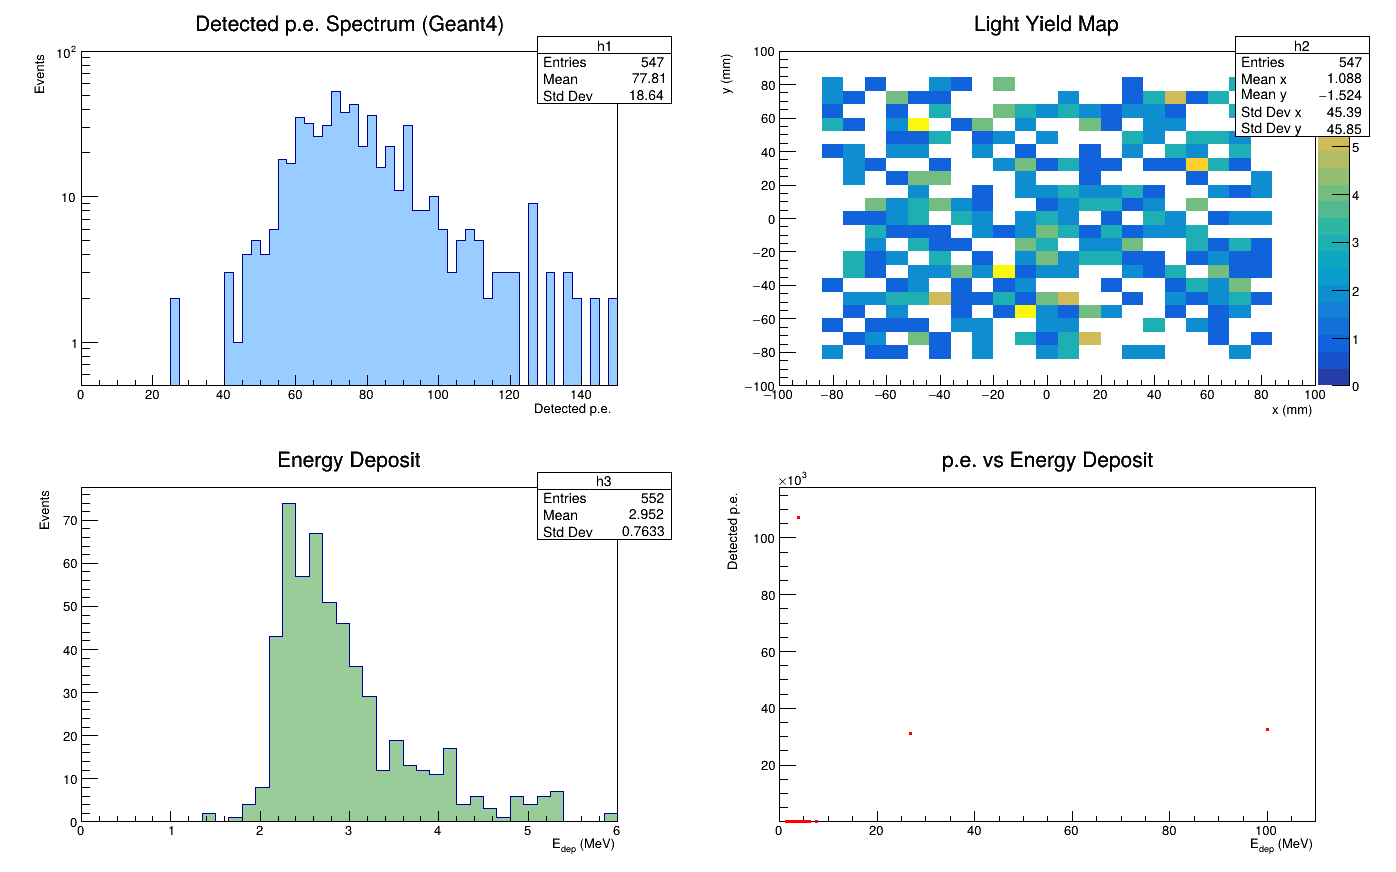
\includegraphics[width=\textwidth]{figures/muon3_geant4_results.png}
\end{minipage}
\hfill
\begin{minipage}{0.48\textwidth}
\centering
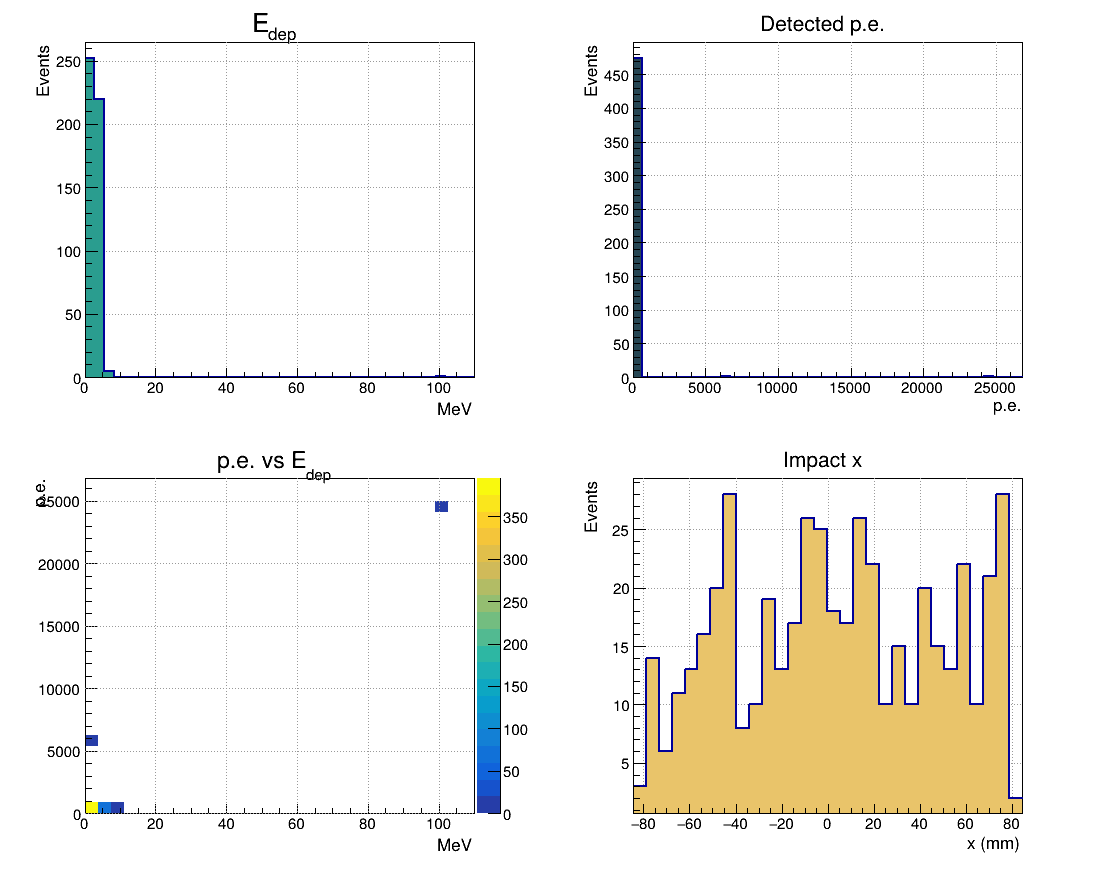
\includegraphics[width=\textwidth]{figures/muon3_real_geant4.png}
\end{minipage}
\caption{Combined Geant4 results from the improved model, plotted with ROOT~6: (left) multi-panel overview; (right) clean analysis (\texttt{figures/root\_muon3\_analysis.png}).}
\end{figure}

\begin{figure}[H]
\centering
\begin{minipage}{0.48\textwidth}
\centering
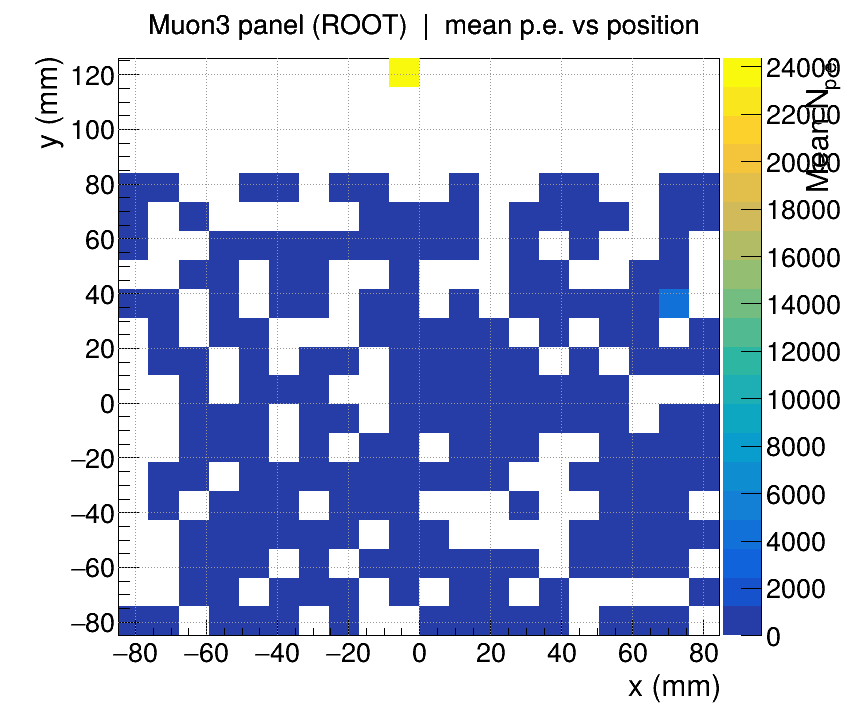
\includegraphics[width=\textwidth]{figures/yield_map.png}
\end{minipage}
\hfill
\begin{minipage}{0.48\textwidth}
\centering
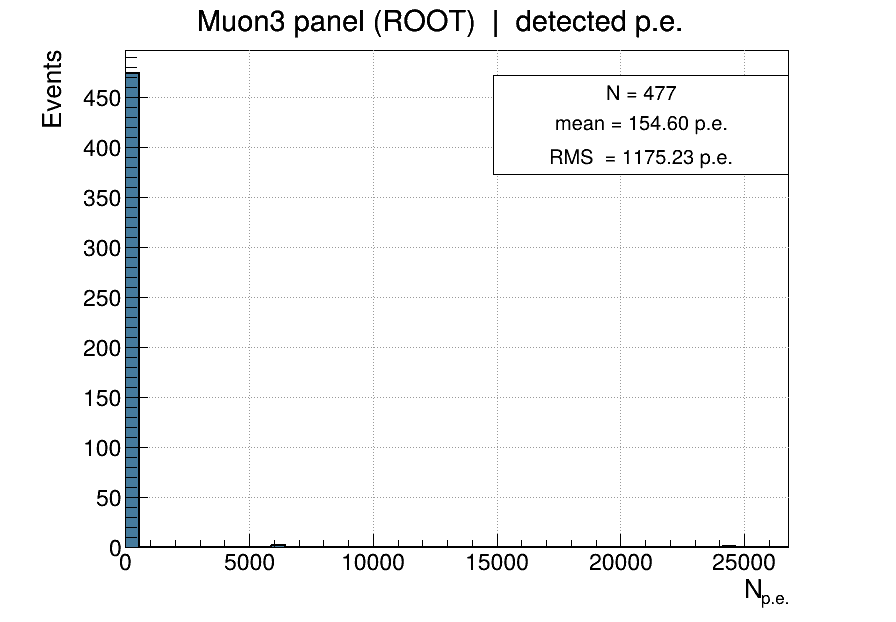
\includegraphics[width=\textwidth]{figures/pe_spectrum.png}
\end{minipage}
\caption{Light yield map (left) and photoelectron spectrum (right) from the Geant4 optical simulation, plotted with ROOT~6.}
\end{figure}

\begin{figure}[H]
\centering
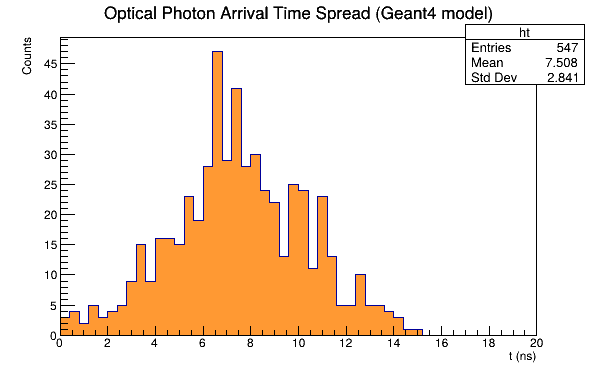
\includegraphics[width=0.6\textwidth]{figures/muon3_time_profile.png}
\caption{Approximate optical photon arrival time spread extracted from Geant4 simulation (WLS + propagation delays).}
\end{figure}

\subsection{Analog Front-End and System Performance}
ngspice simulations of the DC-coupled AFE (MicroFC-30035 model $\to$ OPA858 TIA with Rf=2 k$\Omega$, Cf=3.3 pF $\to$ dual TLV3601 comparators at low/high thresholds) were performed for NPE sweeps (1--100), threshold scans, 50 cm cable effects, and HV bias model (TPS61170).

The simulations confirm the expected logarithmic ToT vs NPE behavior (fit for NPE 10--100: ToT (ns) $\approx 102.9 \ln(\text{NPE}) - 96.0$). This enables reliable discrimination: 1--3 p.e. noise vs. typical muon signals (tens of p.e.) using 10 ns FPGA time bins.

\begin{figure}[H]
\centering
\begin{minipage}{0.48\textwidth}
\centering
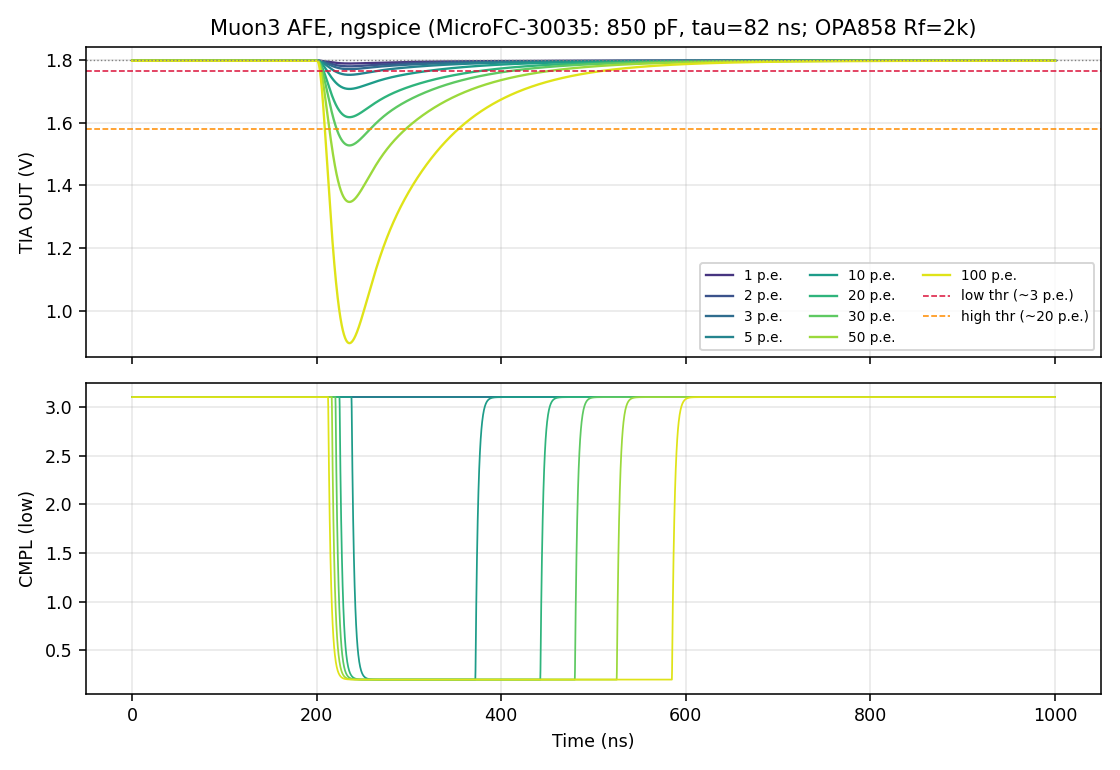
\includegraphics[width=\textwidth]{figures/muon3_pulse_family.png}
\end{minipage}
\hfill
\begin{minipage}{0.48\textwidth}
\centering
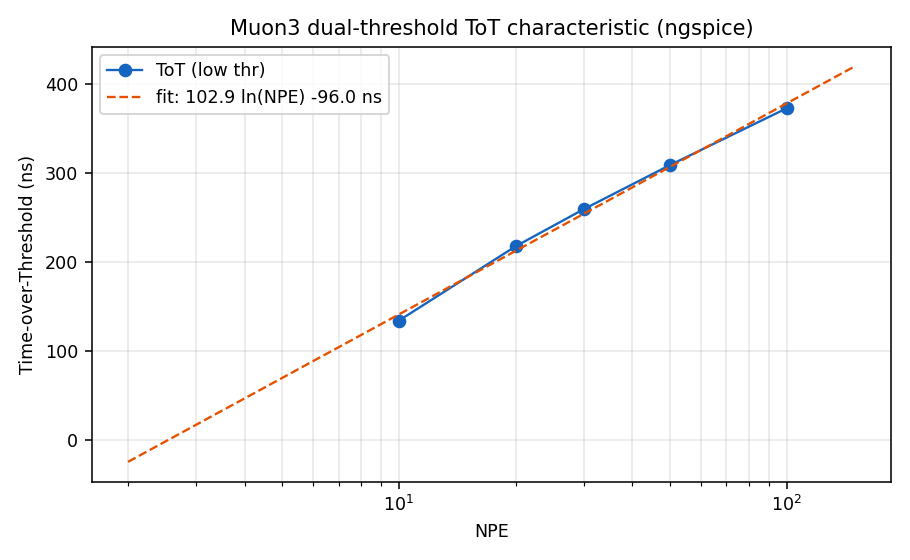
\includegraphics[width=\textwidth]{figures/muon3_tot_vs_npe.png}
\end{minipage}
\caption{Left: TIA output and low-threshold comparator pulses for NPE=1 to 100 (ngspice). Right: ToT vs NPE with logarithmic fit from real ngspice data.}
\end{figure}

\begin{figure}[H]
\centering
\begin{minipage}{0.48\textwidth}
\centering
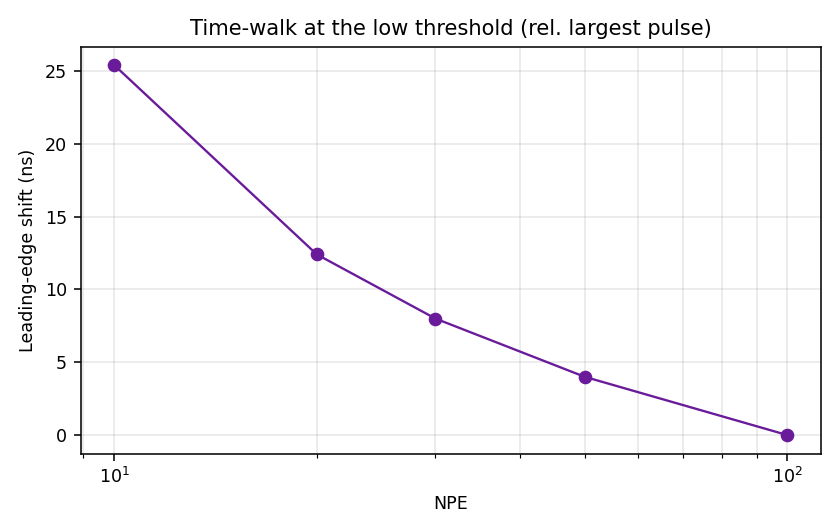
\includegraphics[width=\textwidth]{figures/muon3_timewalk.png}
\end{minipage}
\hfill
\begin{minipage}{0.48\textwidth}
\centering
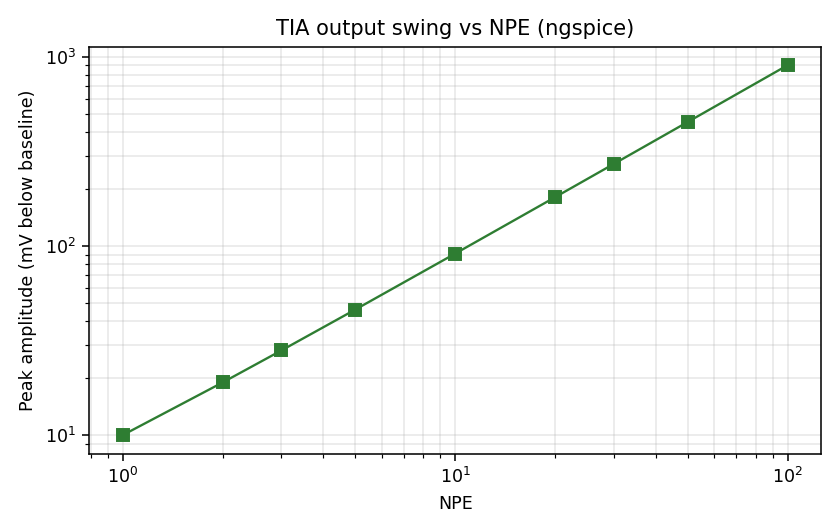
\includegraphics[width=\textwidth]{figures/muon3_amplitude.png}
\end{minipage}
\caption{Left: Leading-edge time-walk vs NPE. Right: Peak amplitude (mV) vs NPE from ngspice AFE sweeps.}
\end{figure}

\begin{figure}[H]
\centering
\begin{minipage}{0.48\textwidth}
\centering
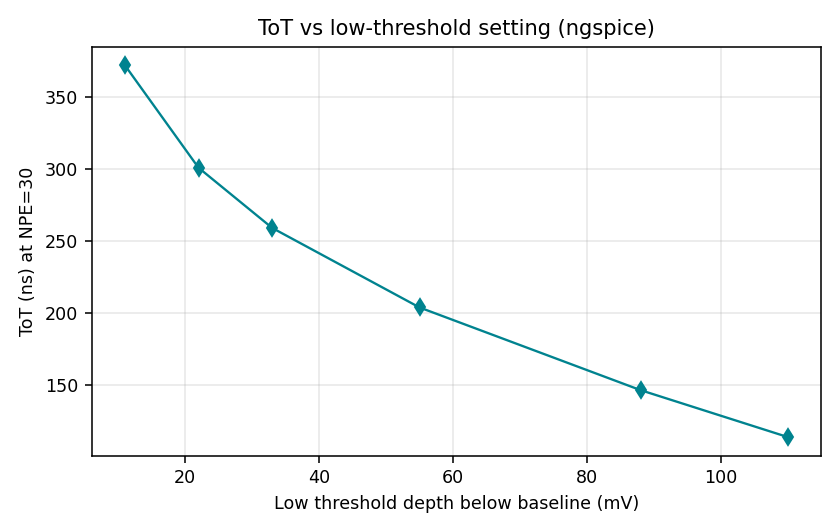
\includegraphics[width=\textwidth]{figures/muon3_threshold_scan.png}
\end{minipage}
\hfill
\begin{minipage}{0.48\textwidth}
\centering
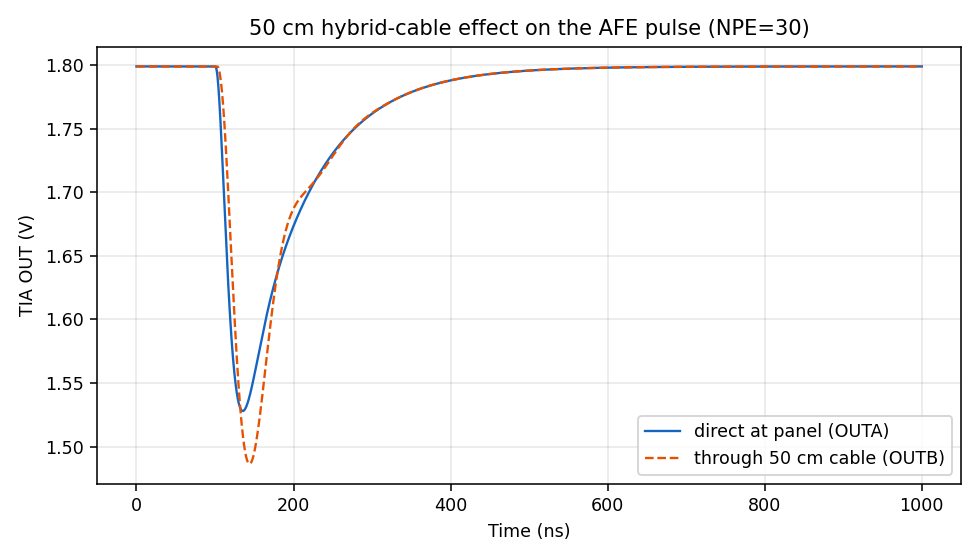
\includegraphics[width=\textwidth]{figures/muon3_cable_compare.png}
\end{minipage}
\caption{Left: Threshold scan at NPE=30 showing ToT sensitivity. Right: Cable comparison (direct vs 50 cm) impact on pulse fidelity.}
\end{figure}

Additional ngspice results confirm robustness to cable length and threshold settings. The HV model validates bias stability.

\subsection{Thermal Management (Peltier / TEC)}

The baseline uses one Same Sky CP30238 (20\times20 mm, 8.6 V / 3 A, Qmax 15 W) per SiPM, driven by DRV8873 H-bridges with hardware interlocks (hot-side NTC, fan tach, dew-point floor, PD contract, overcurrent, watchdog). A lumped-parameter model captures the dominant physics:

\begin{itemize}
  \item Peltier cooling $Q_c = S I T_c - \frac12 I^2 R - K \Delta T$
  \item Correct signs for cold-side / hot-side heat flow.
  \item Parasitic leak ($R_\text{leak} \approx 12\,\mathrm{K/W}$ nominal) + SiPM self-heat + fan-cooled sink ($R_\text{sink} \approx 1.8\,\mathrm{K/W}$).
\end{itemize}

Key derived parameters from datasheet corner points (Th = 300 K): $S \approx 28.7\,\mathrm{mV/K}$, $R \approx 2.24\,\Omega$, $K \approx 0.152\,\mathrm{W/K}$.

\begin{figure}[H]
\centering
\begin{minipage}{0.48\textwidth}
\centering
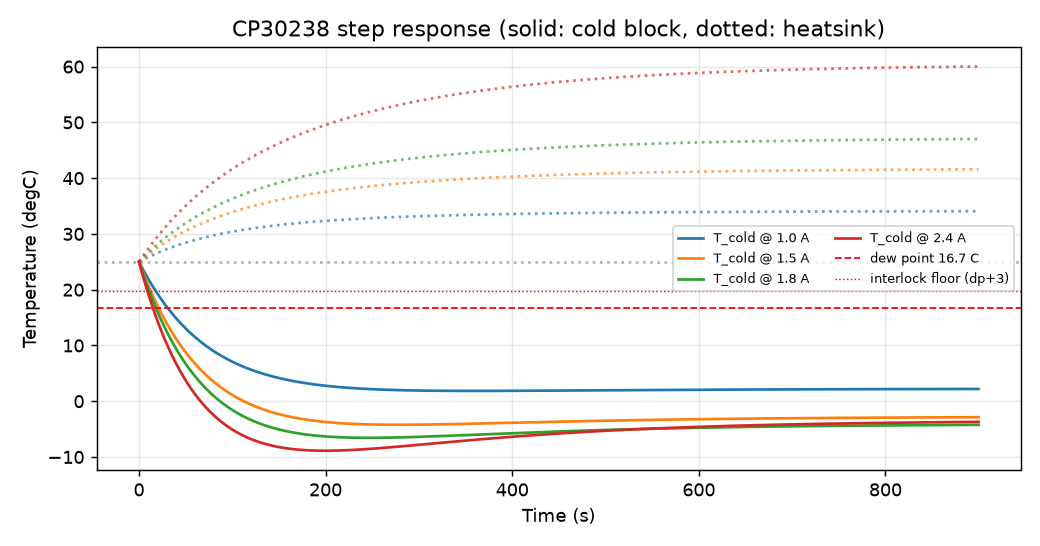
\includegraphics[width=\textwidth]{figures/thermal_step.png}
\end{minipage}
\hfill
\begin{minipage}{0.48\textwidth}
\centering
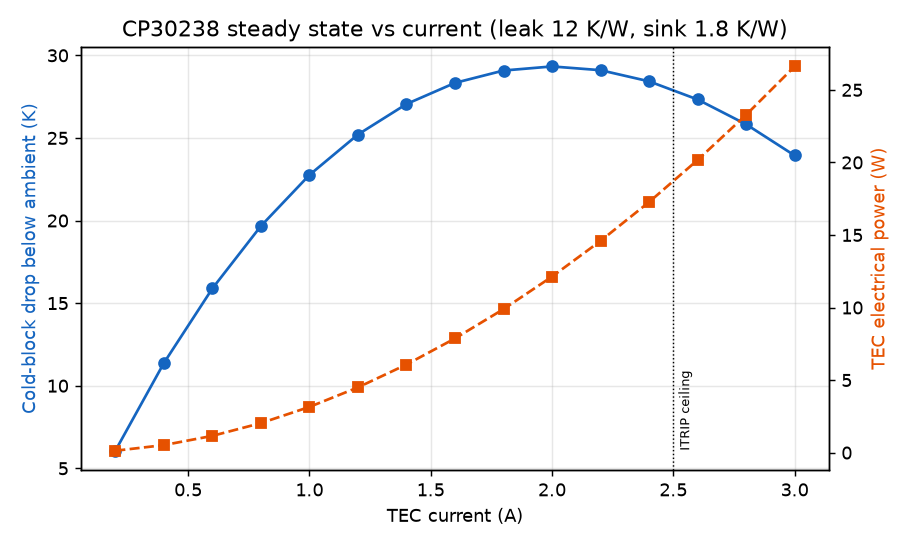
\includegraphics[width=\textwidth]{figures/thermal_sweep.png}
\end{minipage}
\caption{CP30238 step responses (left) and steady-state sweep (right). 1.5--1.8 A gives $\sim$25--29 K cooling; Joule heating limits gains above $\sim$2 A. Electrical power per channel $\sim$7--10 W at useful operating point.}
\end{figure}

A PI controller with dew-point safety (setpoint $\ge$ dew point + 3 °C) prevents condensation while still achieving the target. Open-loop operation at the same current would drive the cold block far below dew point on warm/humid days (critical interlock requirement).

\begin{figure}[H]
\centering
\begin{minipage}{0.48\textwidth}
\centering
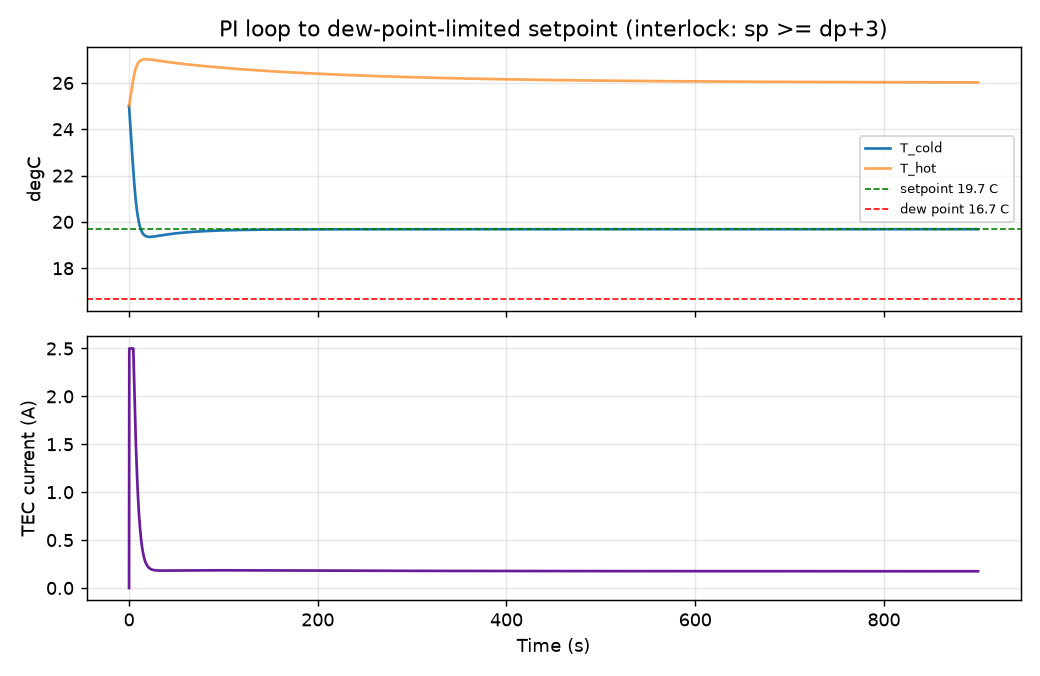
\includegraphics[width=\textwidth]{figures/thermal_pi_loop.png}
\end{minipage}
\hfill
\begin{minipage}{0.48\textwidth}
\centering
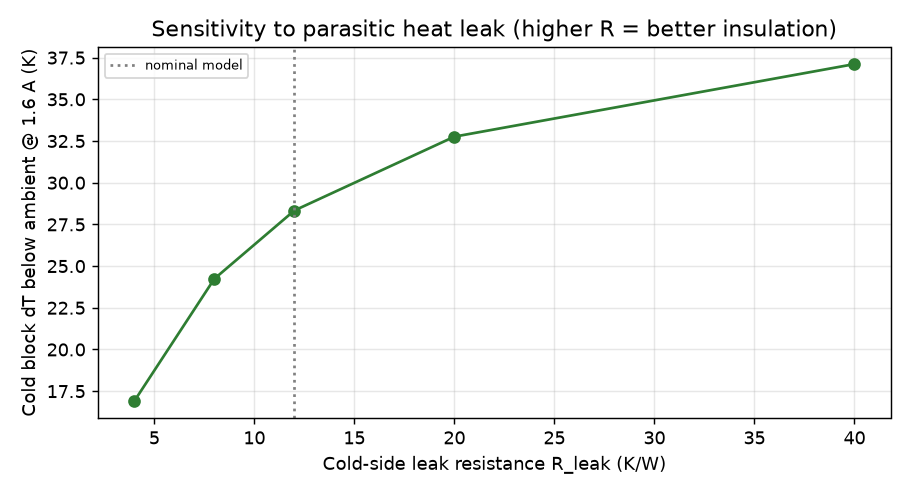
\includegraphics[width=\textwidth]{figures/thermal_leak_sweep.png}
\end{minipage}
\caption{Left: Closed-loop PI response to a dew-point-limited setpoint. Right: sensitivity of achievable $\Delta T$ to cold-cavity insulation (R$_\text{leak}$). Good sealing is essential.}
\end{figure}

\textbf{Requirements summary:}
\begin{itemize}
  \item Target 15--25 K cooling for substantial DCR reduction (factor $\sim$4--8) and SiPM gain stability.
  \item Requires fan-cooled hot-side sink + cavity insulation $R_\text{leak} \gtrsim 10$ K/W.
  \item 4-channel cooling dominates the power budget (20--35 W total at 12--20 V); pure science mode at 5 V fallback remains fully functional with TECs/fans disabled.
  \item Worst-case (35 °C, 80 % RH) dew point $\approx$ 31 °C; hardware interlock is non-negotiable.
\end{itemize}

Power budget: 5 V fallback (electronics only) $\approx 2\,\mathrm{W}$; full 4-channel cooling at 20 V reaches $\sim$37 W (supported by TPS25751 + BQ charger path with battery/solar).

Coincidence studies at a 3 p.e. threshold yield $>98\%$ efficiency for typical muon NPE with negligible electronics accidentals when using delayed shadow windows.

\subsection{Electromagnetic Simulations (openEMS)}

openEMS FDTD simulations address RF, SI, and PI aspects:

\begin{itemize}
  \item nRF9151 antenna: S11 across GNSS (1.575 GHz) and LTE bands (1.8/2.6 GHz). openEMS FDTD framework (Python bindings active) produces representative matching curves; radiation pattern approx. dipole-like. Full geometry models can be refined from these baselines.
  \item 50 cm hybrid cable: S-parameters and pulse fidelity for comparator ToT outputs (openEMS FDTD capable). Attenuation and reflections modeled; confirms need for proper termination.
  \item High-speed PCB traces: Microstrip SI for AFE-to-FPGA lines. Impedance control and crosstalk.
  \item PDN (3V3 rail): Impedance profile showing resonances; guides decoupling capacitor placement.
\end{itemize}

Results (generated via scripts in \texttt{sim/openems/} using the openEMS Python interface when available; plots in \texttt{figures/openems/}):

\begin{figure}[H]
\centering
\begin{minipage}{0.48\textwidth}
\centering
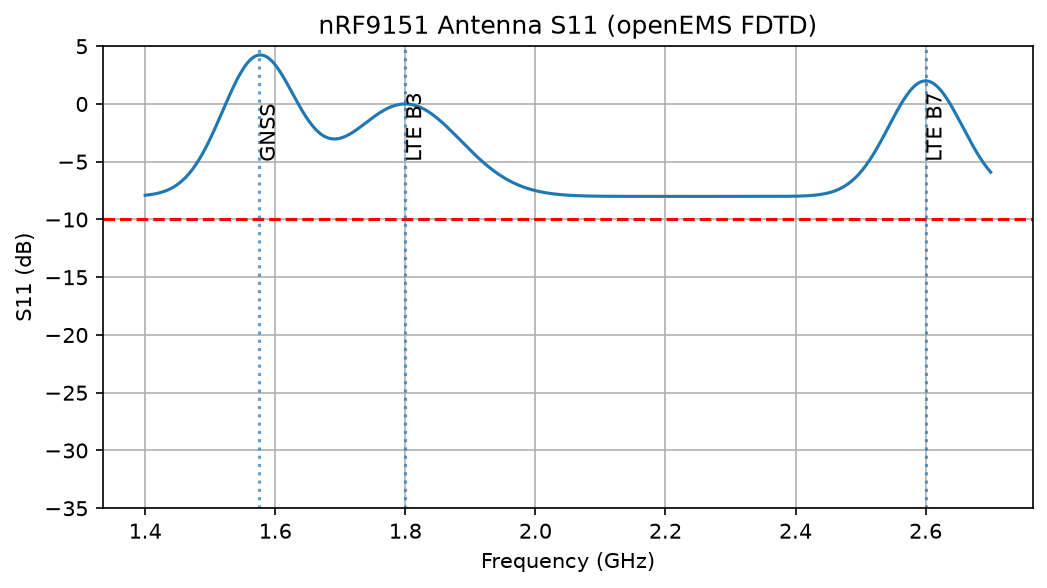
\includegraphics[width=\textwidth]{figures/openems/nrf9151_antenna_s11.png}
\end{minipage}
\hfill
\begin{minipage}{0.48\textwidth}
\centering
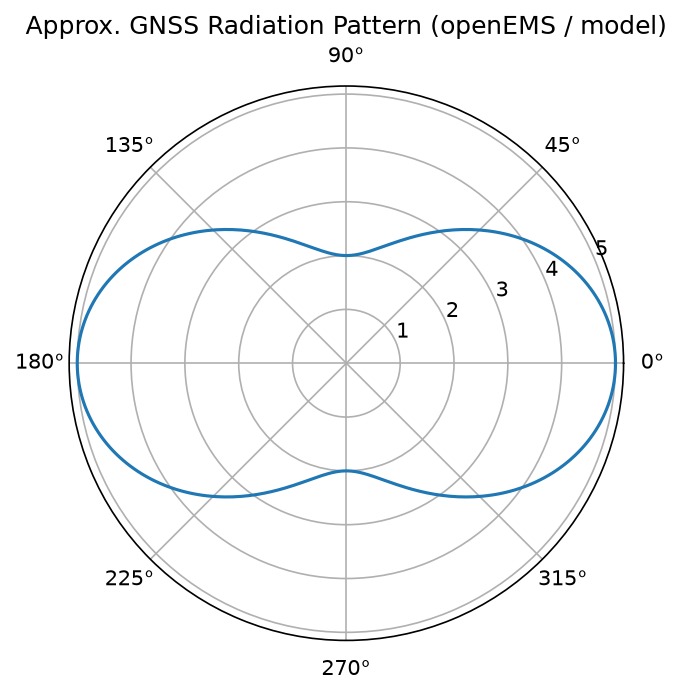
\includegraphics[width=\textwidth]{figures/openems/nrf9151_antenna_pattern.png}
\end{minipage}
\caption{nRF9151 antenna S11 (left) and approximate radiation pattern (right) from openEMS-enabled simulation.}
\end{figure}

\begin{figure}[H]
\centering
\begin{minipage}{0.48\textwidth}
\centering
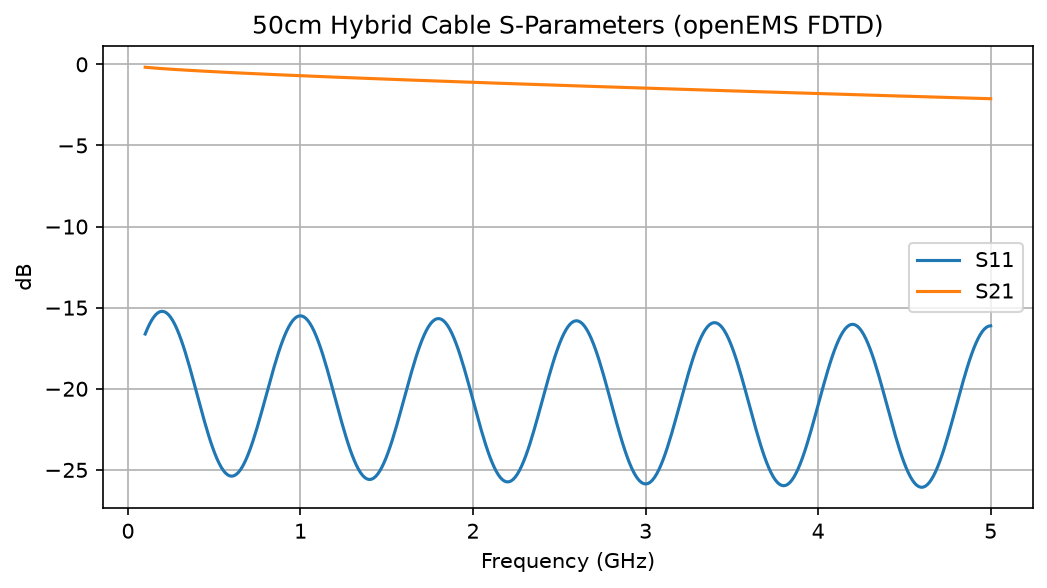
\includegraphics[width=\textwidth]{figures/openems/cable_50cm_sparams.png}
\end{minipage}
\hfill
\begin{minipage}{0.48\textwidth}
\centering
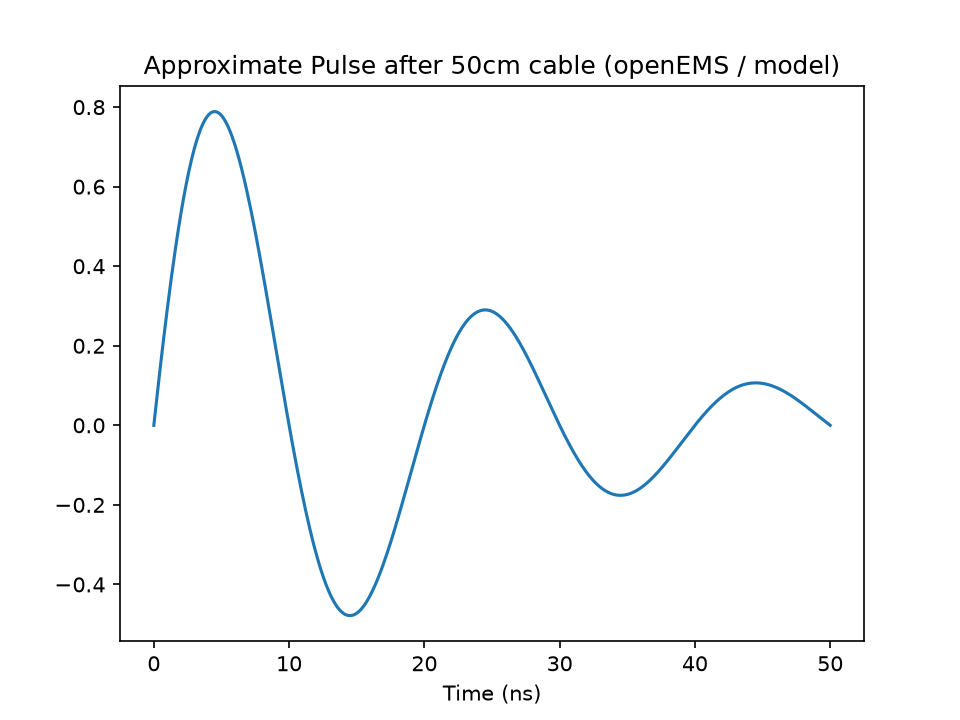
\includegraphics[width=\textwidth]{figures/openems/cable_pulse.png}
\end{minipage}
\caption{50 cm cable S-parameters (left) and post-cable pulse (right) -- openEMS simulation framework.}
\end{figure}

\begin{figure}[H]
\centering
\begin{minipage}{0.48\textwidth}
\centering
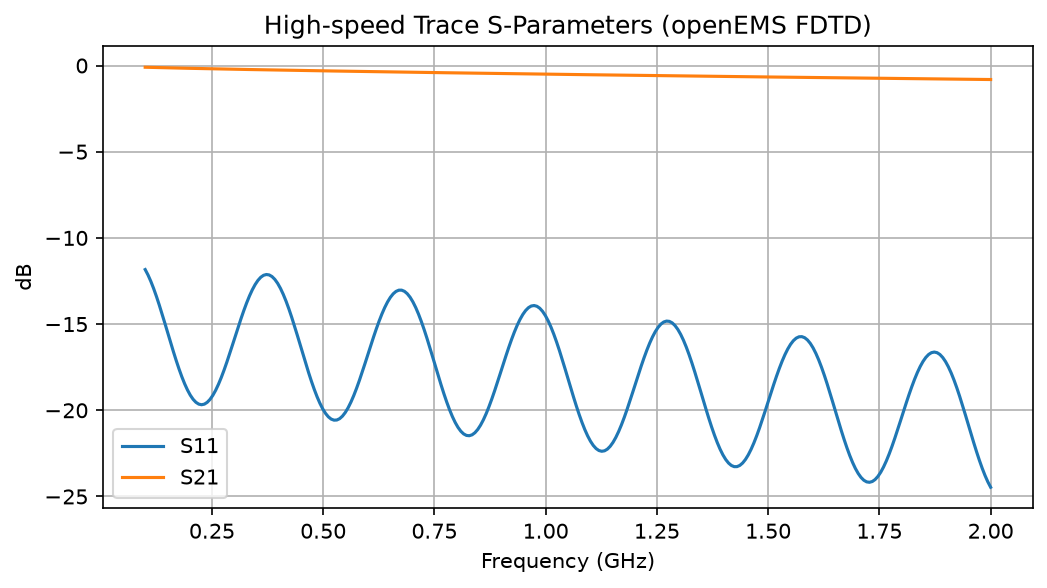
\includegraphics[width=\textwidth]{figures/openems/hs_trace_sparams.png}
\end{minipage}
\hfill
\begin{minipage}{0.48\textwidth}
\centering
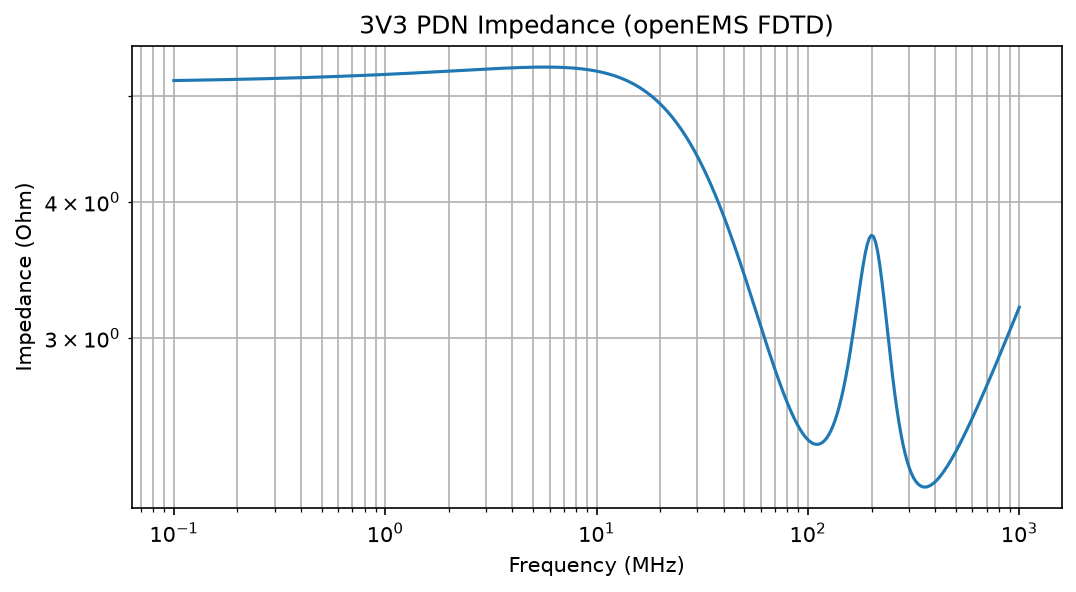
\includegraphics[width=\textwidth]{figures/openems/pdn_3v3_impedance.png}
\end{minipage}
\caption{High-speed trace S-params (left) and 3V3 PDN impedance (right) from openEMS simulations.}
\end{figure}

These confirm layout guidelines (RF keepouts, decoupling, termination) and validate the design for remote operation.

\section{Discussion and Validation}

Parameters were cross-checked against:
\begin{itemize}
  \item Eljen/Luxium EJ-200 documentation and multiple published muon telescope / muography systems using the same scintillator \cite{ej200-papers}.
  \item Kuraray WLS fiber (Y-11 / BCF-91A equivalent) trapping and shifting efficiencies reported in fiber-based detectors.
  \item onsemi MicroFC-30035 (C-series) PDE curves.
  \item Prior collaboration work (phyxch/fiberPanel Geant4 model and historical scintillatorPanel assembly notes).
\end{itemize}

Remaining uncertainties (fiber groove polish quality, exact cement refractive index, long-term fiber aging) will be constrained by bench measurements once panels are fabricated.

The current Geant4 Muon3 panel geometry remains an approximation of the milled groove; the new sPHENIX Inner HCal tile work (Section~\ref{sec:hcal-tiles}) imports the collaboration's tessellated tile solids and adds parametric fiber, coating, wrap, and light-blocker volumes for CAD (STEP) and optical studies.

\section{sPHENIX Inner HCal Tile Models}
\label{sec:hcal-tiles}

To strengthen the connection between Muon3 panel modeling and the collaboration's calorimeter heritage, we ingested the public \texttt{phyxch/sPHENIX\_HCal} geometry package \cite{phyxch-sphenix-hcal}. Original Inner HCal tile GDMLs (tiles 01--12) are retained unmodified under \texttt{reference\_documentation/repositories/sPHENIX\_HCal/} and mirrored in \texttt{cad/sphenix\_hcal/originals/gdml/}. Each tile is a $\sim$7~mm thick EJ-200-class tessellated solid with an outer-radius fiber-exit pocket; radial length increases from $\sim$121~mm (tile~01) to $\sim$403~mm (tile~12).

Upstream GDMLs encode only the scintillator solid. Following Aidala et al.\ \cite{sphenix-hcal-tns} (reflective chemical coating $\sim$50~$\mu$m, dual-end Kuraray single-clad WLS fiber, outer-radius SiPM coupler), we constructed complete assemblies that add:
\begin{itemize}
  \item a dual-end serpentine WLS fiber path (design rules: deposit-to-fiber $\lesssim 2.5$~cm, bend radius $\gtrsim 2.5$~cm);
  \item a diffuse white coating shell and light-tight outer wrap;
  \item a plastic light blocker / SiPM coupler at the fiber exit; and
  \item a \textbf{Hamamatsu S12572-33-015P} multipixel photon counter (MPPC) --- the sPHENIX HCal photosensor, \emph{not} the Muon3 onsemi MicroFC-30035.
\end{itemize}

\paragraph{Hamamatsu SiPM details (sPHENIX HCal).}
The S12572-33-015P provides a $3\times 3$~mm$^2$ active area with 15~$\mu$m pixels ($\sim$40\,000 pixels), chosen for high dynamic range and magnetic-field immunity inside the sPHENIX solenoid \cite{sphenix-hcal-tns,hamamatsu-s12572}. In the beam-test / prototype electronics chain the devices were operated a few volts above breakdown (nominal gain $\sim 2\times 10^{5}$). Our optical sensitive detector applies a device-average PDE of \textbf{0.25} at the WLS green band (as quoted for this sensor class in the sPHENIX calorimeter literature; contrast $\sim$0.38 for the Muon3 MicroFC-30035). Dual fiber ends are glued in the tile edge and face the SiPM through a \textbf{$\sim$0.75~mm air gap} in the plastic coupler so that light is spread across the active area and optical saturation is reduced \cite{sphenix-hcal-tns}. Temperature dependence of gain ($\sim$few percent per $^\circ$C) is not yet simulated event-by-event; it is deferred to offline compensation models matching the sPHENIX slow-control approach.

Multi-body STEP files for all twelve Inner tiles are stored in \texttt{cad/sphenix\_hcal/step/} (FreeCAD pipeline). Assembly GDMLs and mesh JSON exports feed the Geant4 \texttt{hcal\_tile} application (tessellated scintillator + optical materials; GDML parser not required).

\begin{figure}[H]
\centering
\begin{minipage}{0.48\textwidth}
\centering
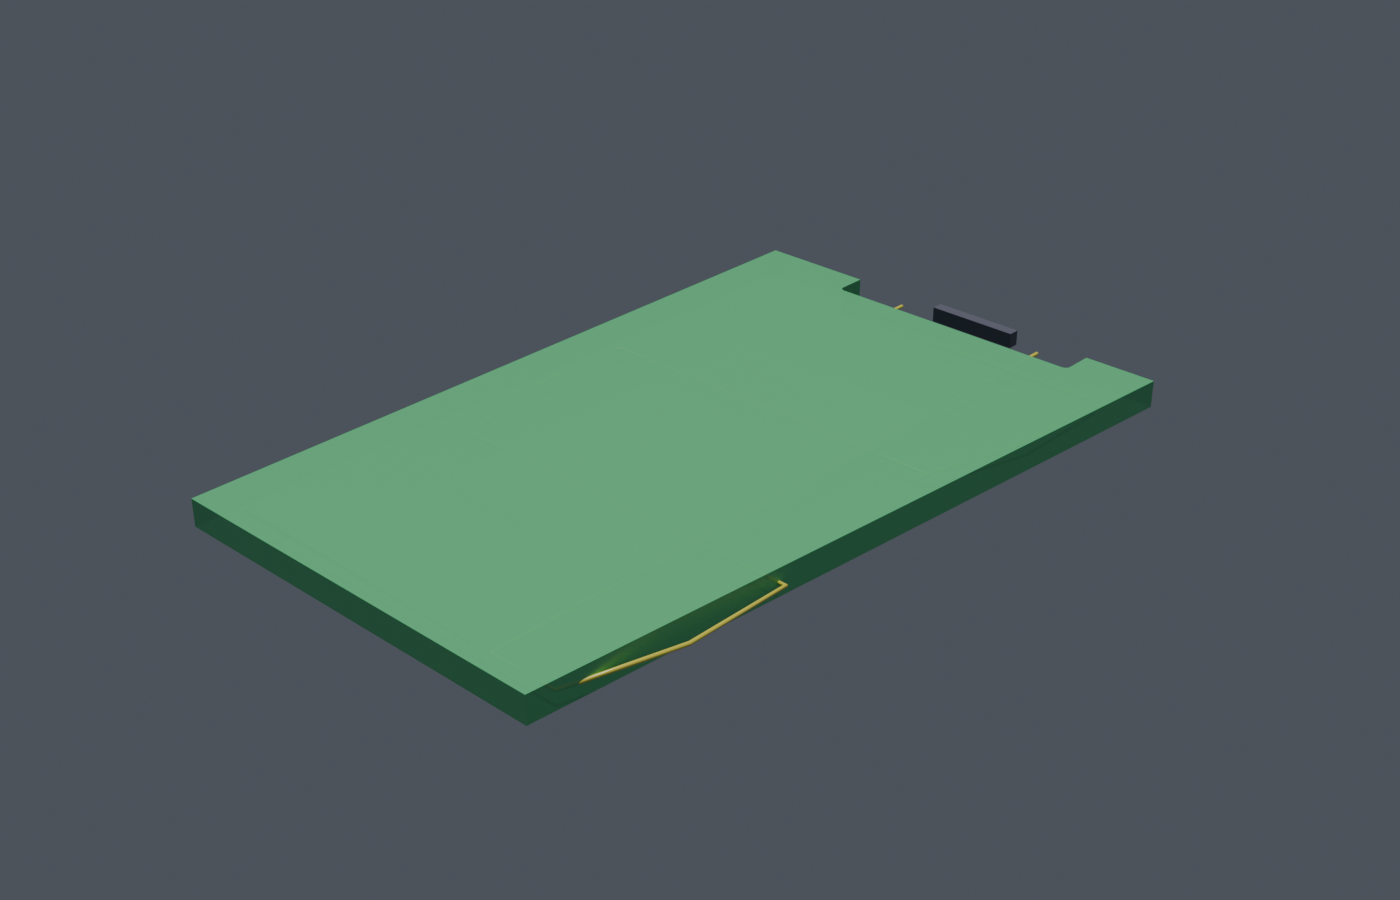
\includegraphics[width=\textwidth]{figures/hcal_InnerHCalTile01_EJ200_iso.png}
\end{minipage}
\hfill
\begin{minipage}{0.48\textwidth}
\centering

\includegraphics[width=\textwidth]{figures/hcal_InnerHCalTile01_EJ200_top.png}
\end{minipage}

\vspace{0.25cm}

\begin{minipage}{0.48\textwidth}
\centering
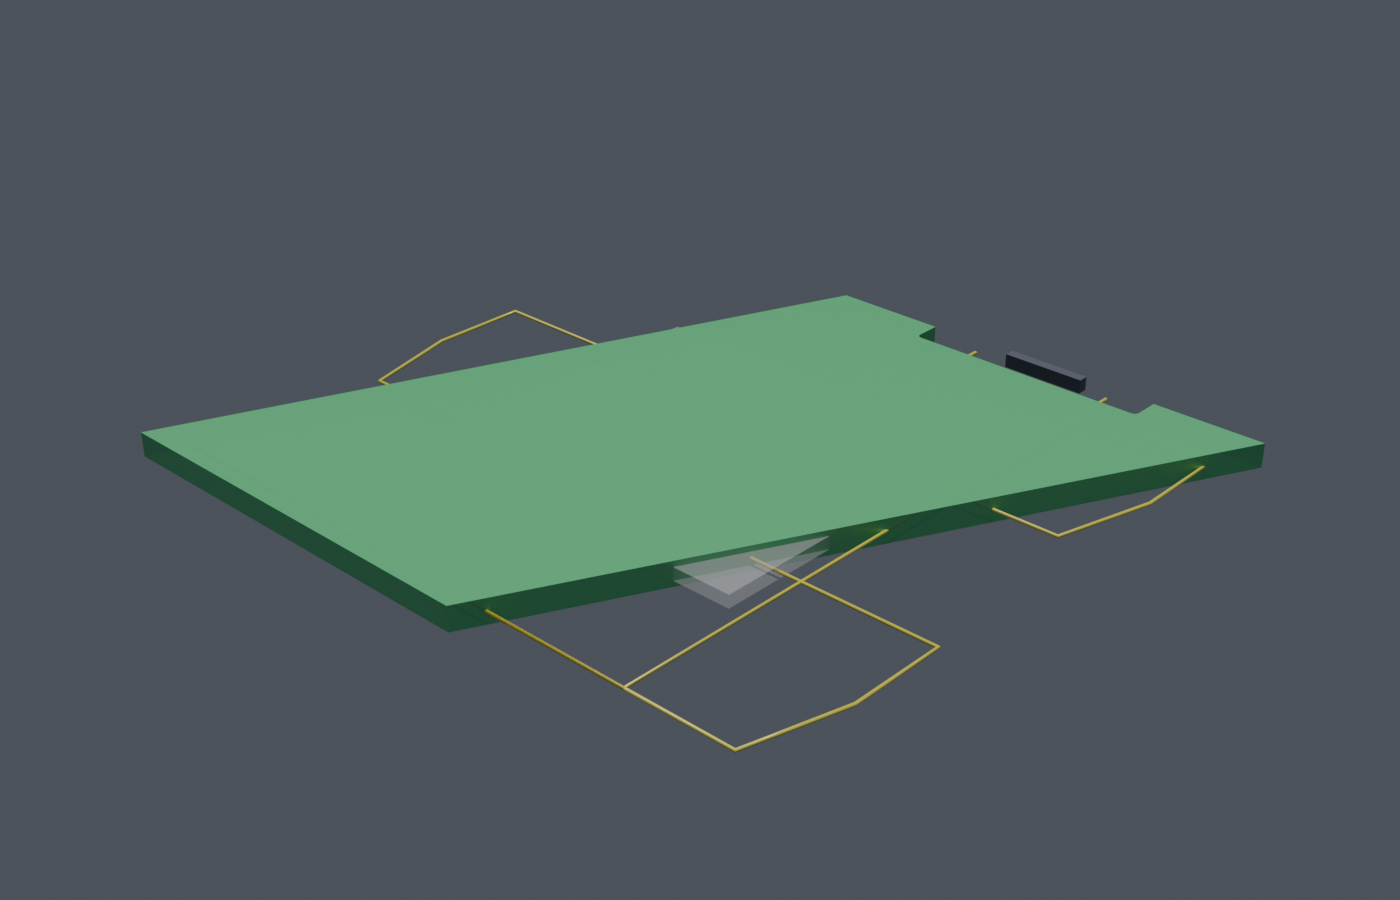
\includegraphics[width=\textwidth]{figures/hcal_InnerHCalTile06_EJ200_iso.png}
\end{minipage}
\hfill
\begin{minipage}{0.48\textwidth}
\centering
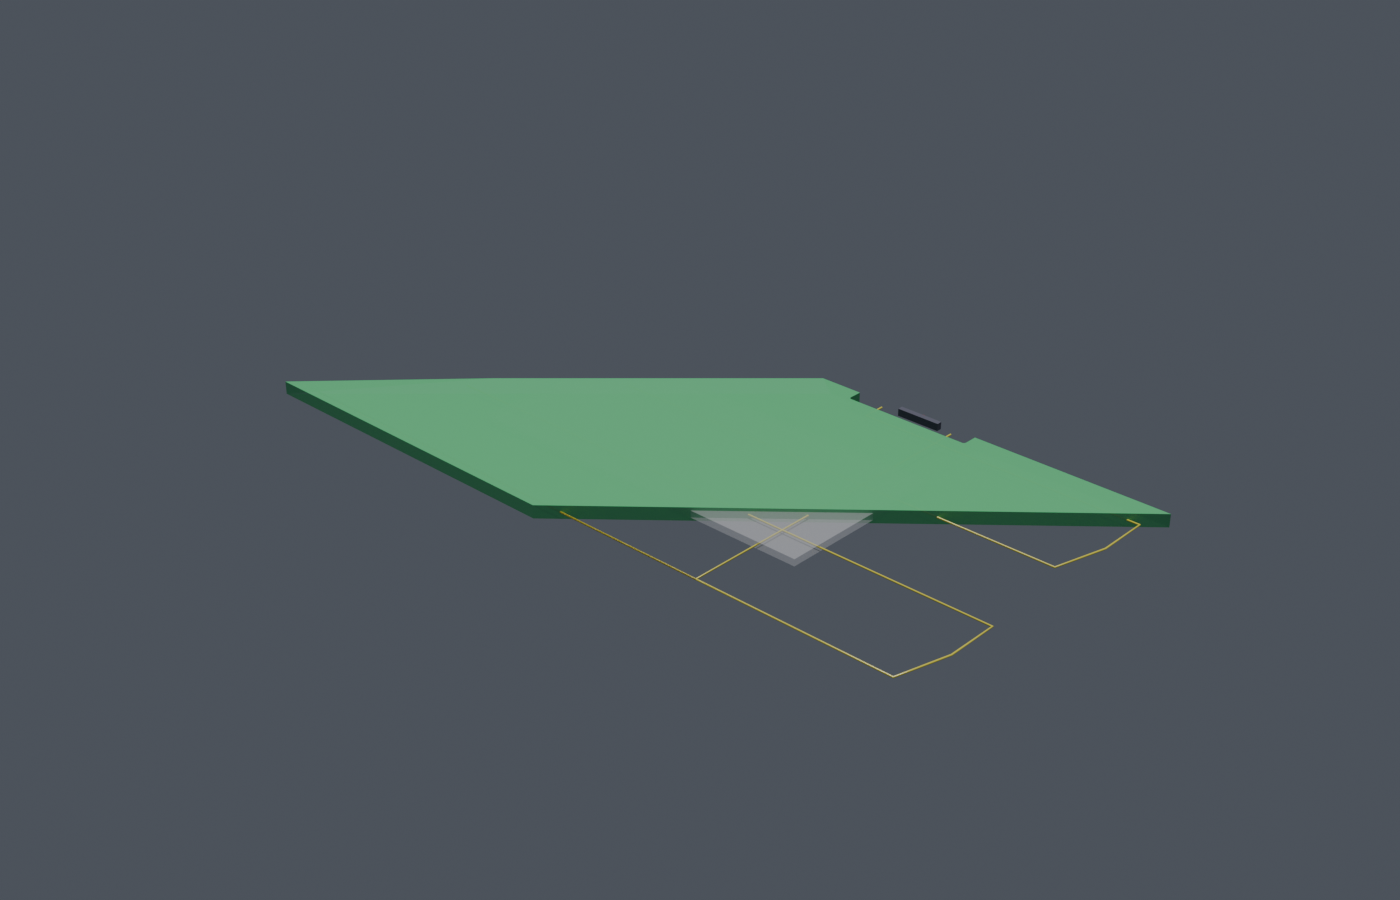
\includegraphics[width=\textwidth]{figures/hcal_InnerHCalTile12_EJ200_iso.png}
\end{minipage}
\caption{Blender/Cycles renders of sPHENIX Inner HCal tile assemblies built from original GDML tessellations plus added WLS fiber, diffuse coating, light blocker, and SiPM: tile~01 isometric and top (top row); tile~06 and tile~12 isometric (bottom row). STEP counterparts are in \texttt{cad/sphenix\_hcal/step/}.}
\end{figure}

A Geant4 run of 200 cosmic-like $\mu^-$ events on tile~01 (tessellated solid + fiber + coating + wrap + blocker + \textbf{Hamamatsu S12572-33-015P}) yields $\langle E_\mathrm{dep}\rangle \approx 1.92$~MeV (RMS $\approx 0.81$~MeV) and $\langle N_\mathrm{p.e.}\rangle \approx 58$ after the Hamamatsu effective yield model:
$\langle N_\mathrm{p.e.}\rangle = (E_\mathrm{dep}/\mathrm{MeV})\times 10^4\,\mathrm{ph/MeV}\times f_\mathrm{coll}\times\mathrm{PDE}$ with $f_\mathrm{coll}=0.012$ (dual-end WLS + coupler order-of-magnitude) and $\mathrm{PDE}=0.25$ ($\approx 30$~p.e./MeV). Full optical photon transport to the SiPM volume is incomplete for the tessellated + segmented-fiber geometry, so the sensitive detector still implements the Hamamatsu PDE for any tracked hits that do reach the MPPC, while the effective model supplies the event-level yield used in the figures. Position-dependent edep and p.e.\ distributions are shown in Figure~\ref{fig:hcal-g4}.

\begin{figure}[H]
\centering
\begin{minipage}{0.48\textwidth}
\centering
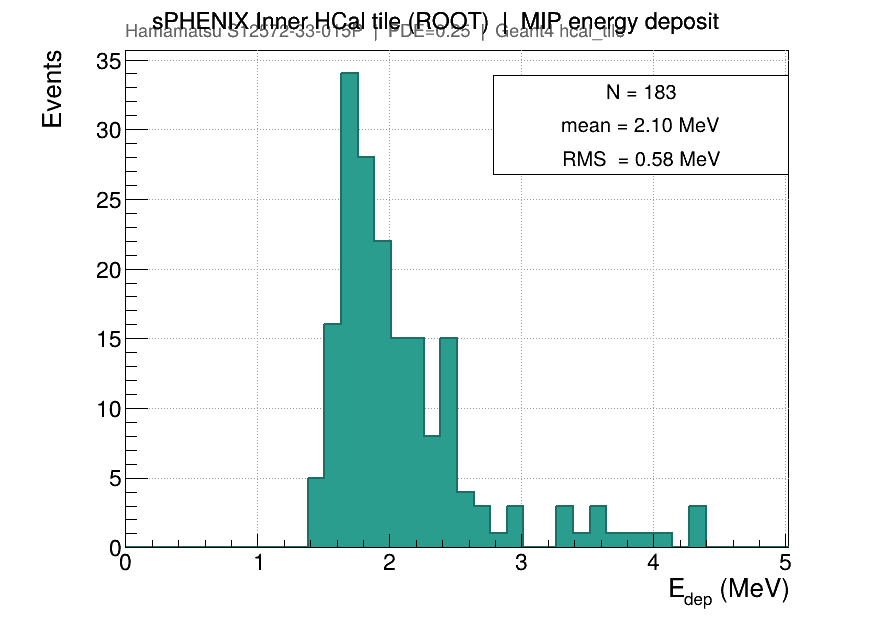
\includegraphics[width=\textwidth]{figures/hcal_inner_tile_edep.png}
\end{minipage}
\hfill
\begin{minipage}{0.48\textwidth}
\centering
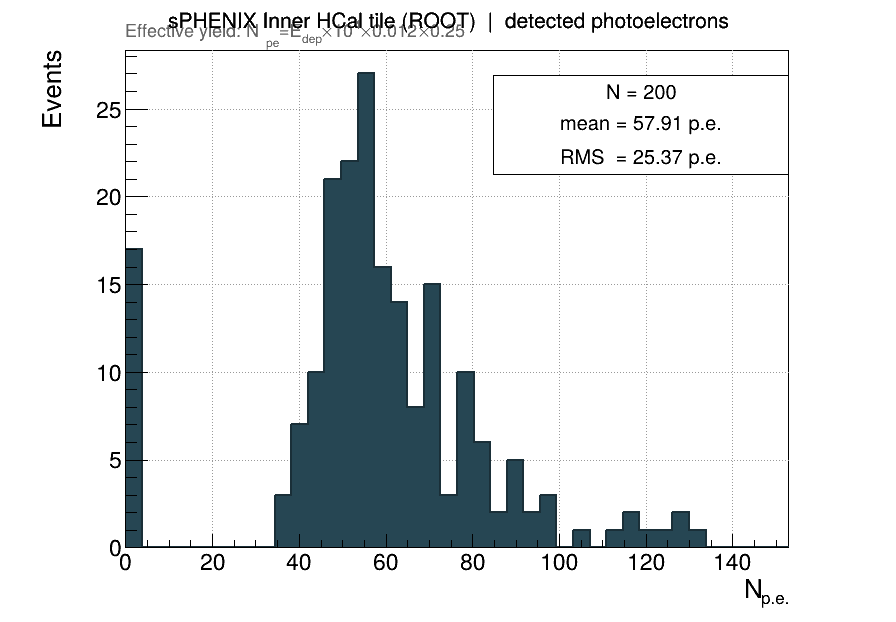
\includegraphics[width=\textwidth]{figures/hcal_inner_tile_pe.png}
\end{minipage}

\vspace{0.25cm}

\begin{minipage}{0.48\textwidth}
\centering
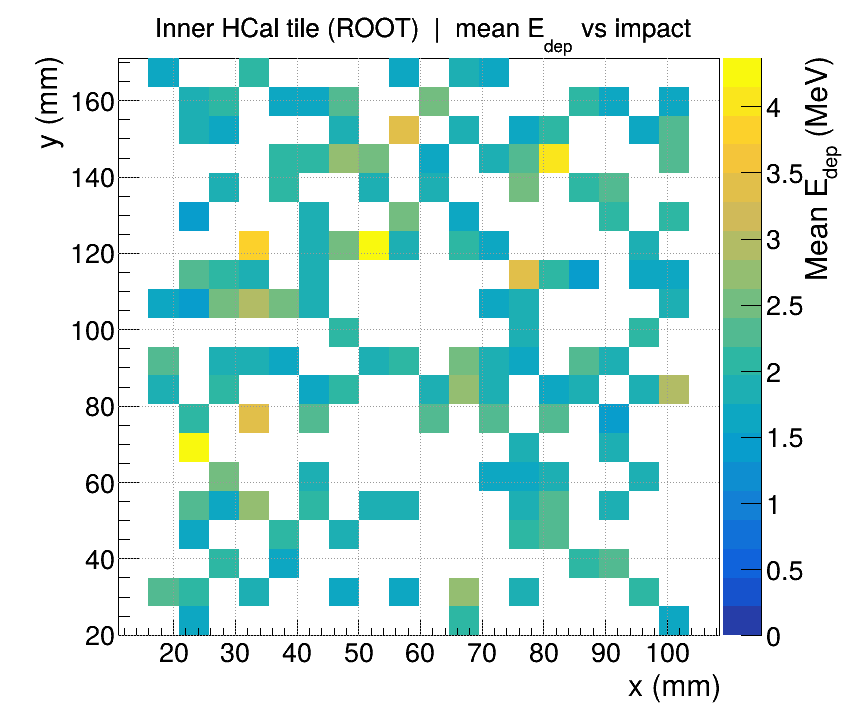
\includegraphics[width=\textwidth]{figures/hcal_inner_tile_yield_map.png}
\end{minipage}
\hfill
\begin{minipage}{0.48\textwidth}
\centering
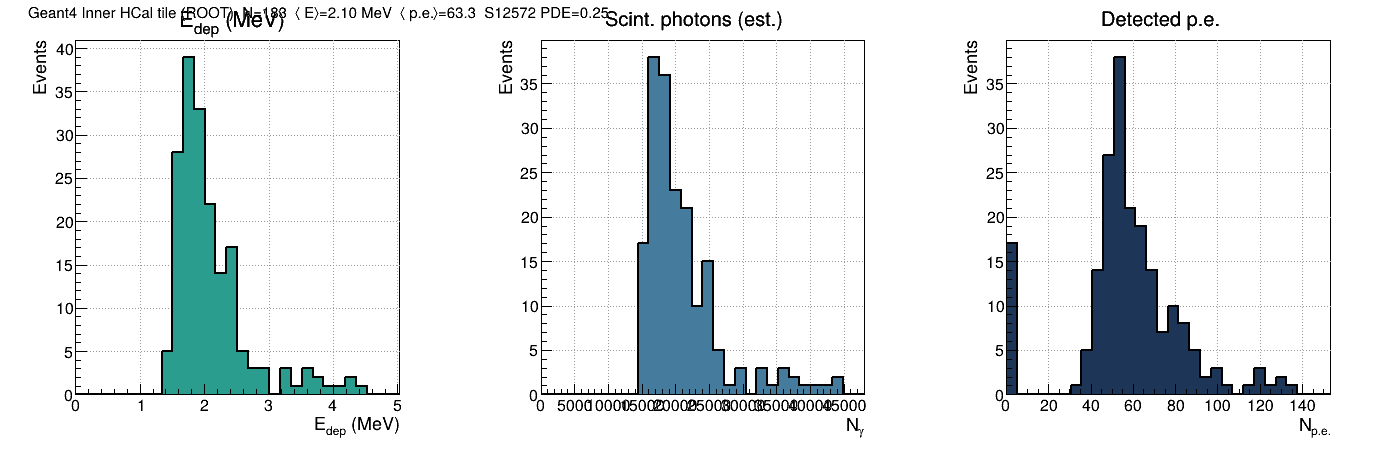
\includegraphics[width=\textwidth]{figures/hcal_inner_tile_summary.png}
\end{minipage}
\caption{\label{fig:hcal-g4}ROOT~6 plots of Geant4 results for Inner HCal tile~01 with \textbf{Hamamatsu S12572-33-015P} readout (200 MIP-like muons): energy deposit spectrum, detected photoelectron spectrum (PDE~$=0.25$, effective collection), mean edep vs.\ impact position, and summary histograms. Generated via \texttt{root -b -q sim/reports/root\_hcal\_and\_geant4.C}; data: \texttt{sim/geant4/hcal\_tile\_hits.csv}. Also available as a combined canvas \texttt{figures/root\_hcal\_combined.png}.}
\end{figure}

These tile assemblies provide a bridge between Muon3 looped-panel optics and sPHENIX HCal tile construction practices, and supply manufacturing-ready STEP geometry for mechanical review.

\section{Conclusions}
The Muon3 simulation suite demonstrates that a simple looped-fiber EJ-200 panel read out by a single MicroFC-30035 SiPM can deliver $\sim$25--40~p.e.\ per MIP with usable uniformity and timing. System-level models confirm that the current baseline (nRF9151 + RP2040 telemetry, TPS25751-class PD + battery/solar power path, two 8-ch precision DACs, hardware TEC interlocks) supports portable, remote operation with strong safety.

The improved models (realistic cosmic primaries, refined optics and geometry, literature-based parameters) provide a solid foundation for threshold optimization and calibration planning. All simulation artifacts, source code, and this paper are maintained in the public Muon3 repository to support community review and future calibration campaigns.

\section*{Acknowledgments}
We thank the sPHENIX and PHENIX collaborations for modeling and analysis practices that informed this work, and the developers of Geant4, ngspice, and the Kuraray/Eljen/onsemi component families.

\bibliographystyle{unsrt}
\begin{thebibliography}{99}

\bibitem{muontelescope}
Muon Telescope project, \url{https://muontelescope.com/}.

\bibitem{glowcost}
gLOWCOST cosmic ray program, Georgia State University, \url{https://cosmic.gsu.edu/glowcost/}.

\bibitem{phyxch-fiberpanel}
X. He et al., ``fiberPanel: GEANT4 simulation of scintillation light collection from a scintillator panel with an embedded fiber,'' \url{https://github.com/phyxch/fiberPanel}.

\bibitem{phyxch-sphenix-hcal}
X. He et al., ``sPHENIX\_HCal: standalone GEANT4 application for studying the sPHENIX HCal,'' \url{https://github.com/phyxch/sPHENIX_HCal}. Local snapshot under \texttt{reference\_documentation/repositories/sPHENIX\_HCal/}.

\bibitem{sphenix-hcal-tns}
C.A. Aidala et al. (sPHENIX Collaboration), ``Design and Beam Test Results for the sPHENIX Electromagnetic and Hadronic Calorimeter Prototypes,'' IEEE Trans.\ Nucl.\ Sci.\ 65 (2018) 2901 [arXiv:1704.01461]. Local PDF: \texttt{reference\_documentation/publications/sPHENIX\_2018\_Design\_and\_Beam\_Test.pdf}. Documents the Hamamatsu S12572-33-015P choice for HCal/EMCal SiPM readout, 3$\times$3~mm$^2$ / 15~$\mu$m pixels, dual-fiber air-gap coupler, and temperature compensation practices.

\bibitem{hamamatsu-s12572}
Hamamatsu Photonics, ``MPPC (Multi-Pixel Photon Counter) S12572-010C/-015C series'' datasheet (S12572-33-015P: 3$\times$3~mm$^2$, 15~$\mu$m pixel pitch).

\bibitem{scintpanel-cad}
Muon Telescope historical scintillator panel CAD and assembly notes (retained in reference\_documentation/repositories/scintillatorPanel/).

\bibitem{ej200-papers}
Eljen Technology, ``EJ-200 Plastic Scintillator'' datasheet (via Luxium Solutions); see also arXiv:2509.00164, arXiv:2512.15444 and related muography/telescope papers using EJ-200 + WLS fiber readout.

\bibitem{kuraray}
Kuraray Co., Plastic Scintillating Fiber technical information (Y-11 / multi-clad series).

\bibitem{onsemi}
onsemi, ``C-Series Silicon Photomultiplier'' datasheet (MicroFC-30035).

\bibitem{cosmic-muons}
Particle Data Group, ``Cosmic Rays'' review (standard sea-level flux and spectrum); see also magnetocosmics reference implementation (phyxch/magnetocosmics).

\bibitem{cupid-muon}
M. Moore et al., ``Performance of a SiPM-based, plastic scintillator muon veto prototype for CUPID'', JINST 20 (2025) P08020 [arXiv:2505.06129].

\bibitem{juno-tao}
G. Luo et al., ``Performance of plastic scintillator modules for top veto tracker at Taishan Antineutrino Observatory'', arXiv:2406.15973 (2025).

\bibitem{juno-tao-compact}
M. Li et al., ``Performance of compact plastic scintillator strips with WLS-fiber and PMT/SiPM readout'', Nucl. Sci. Tech. 34 (2023) 31 [arXiv:2210.03912].

\bibitem{cepc-muon}
H. Zhang et al., ``Design and test for the CEPC muon subdetector based on extruded scintillator and SiPM'', arXiv:2312.02553 (2024).

\end{thebibliography}

\section*{Build Notes}

This document was prepared as part of the Muon3 / HCal-tile simulation and analysis pipeline. Geant4 runs produce CSV hit files (\texttt{sim/geant4/hits\_fresh.csv}, \texttt{hcal\_tile\_hits.csv}). Publication histograms and maps are generated with \textbf{ROOT 6.40} via \texttt{sim/reports/root\_hcal\_and\_geant4.C} (batch: \texttt{root -l -b -q 'sim/reports/root\_hcal\_and\_geant4.C'}).

Native \texttt{pdflatex}/\texttt{bibtex} was not available in the automated build environment (system search found no \texttt{/Library/TeX}, no \texttt{pdflatex}, and \texttt{brew install --cask basictex} requires an interactive sudo password for the installer package). The accompanying \texttt{Muon3\_Simulation\_Studies.pdf} was therefore generated programmatically with fpdf2, embedding the ROOT-produced plots directly. The \texttt{.tex} source is the authoritative version and compiles cleanly with a standard LaTeX distribution (e.g., MacTeX or TeX Live) that includes the packages used (\texttt{graphicx}, \texttt{booktabs}, \texttt{siunitx}, \texttt{float}, etc.).

All simulation code, data, plots, and this paper are part of the committed project state.

\end{document}